\section{Analysis of the frequency domain EM response of a conductive, permeable well}
\label{app:fdem}

\subsection{Currents in the formation}
We consider the EM response of a conductive, permeable casing in a frequency domain EM experiment. We use the same survey geometry and physical properties as shown in Figure \ref{fig:setup}, and now consider a harmonic waveform. We again begin by examining the currents in the subsurface and show the real component of the currents in Figure \ref{fig:fdem-cross-section-currents-real} for (a) a halfspace model, (b) a conductive casing ($\sigma = 5\times10^6$ S/m, $\mu=\mu_0$), (c) a conductive, permeable casing ($\sigma = 5\times10^6$ S/m, $\mu=150\mu_0$), and (d) the anomalous currents due to the permeability of the casing. For frequencies up to 10Hz, the response is visually identical to the DC response we observed in Figure \ref{fig:tdem-cross-section-currents}. This is to be expected, at the resistive limit of Maxwell's equations, the EM response is dominated by the galvanic currents. At higher frequencies, we can see the effects of induction for all of the models with the development of current systems at depth that circulate in a direction opposite to the galvanic currents.


\begin{figure}
    \begin{center}
    \includegraphics[width=\textwidth]{figures/fdem-cross-section-currents-real.png}
    \end{center}
\caption{Cross sections of the real component of the current density in frequency domain EM experiments over (a) a half-space, (b) a conductive well ($5\times10^6$ S/m, $\mu_0$), and (c) a conductive, permeable well ($5\times10^6$ S/m, $150\mu_0$). The panel on the right shows (d) the difference between the conductive, permeable well and the conductive well.
}
\label{fig:fdem-cross-section-currents-real}
\end{figure}





A benefit of working in the frequency domain as compared to the time domain is that it is simpler to isolate the inductive component of a response. In the time domain, after the transmitter is turned off, both the galvanic and image current-systems diffuse downwards and outwards through time, so there is no straightforward way to separate them. However, in the frequency domain, where the transmitter is always on, the geometry of the galvanic portion of the response remains the same at all frequencies. Thus, we can isolate the inductive response in the real component by subtracting off the response at the DC limit (0 Hz). This is what is shown in Figure \ref{fig:fdem-cross-section-currents-subtract-dc}.

Isolating the inductive component of the real response provides a useful connection to our analysis in the time-domain. The geometry of currents resembles those observed in the time-domain, where time and frequency are inversely related. Note that the arrows are in the opposite direction; this is a function of the choice of an $e^{i\omega t}$ Fourier transform convention that follows \citep{Ward1988}. Our choice of Fourier transform convention is somewhat inconvenient for making comparisons between the time and frequency domains, because of the sign reversal, however, we chose to use this convention because it is common in geophysics and is the convention that is implemented in SimPEG.

\begin{figure}
    \begin{center}
    \includegraphics[width=\textwidth]{figures/fdem-cross-section-currents-subtract-dc.png}
    \end{center}
\caption{
    Cross sections of the inductive part of the real current density (real component of the current density minus the DC current density).
}
\label{fig:fdem-cross-section-currents-subtract-dc}
\end{figure}





In Figure \ref{fig:fdem-cross-section-currents-imag}, we show the imaginary component of the currents. The geometry is similar to the inductive component of the real response in Figure \ref{fig:fdem-cross-section-currents-subtract-dc}, but in the imaginary component, we also see the influence of the magnetic field. The ``flattening'' of the currents beneath the transmitter wire (x=0m to x=1000m) is a result of the rotational magnetic field created by the transmitter according to Ampere's law. In both Figures \ref{fig:fdem-cross-section-currents-subtract-dc} and \ref{fig:fdem-cross-section-currents-imag}, we see the ``shadow-zone'' that is responsible for the zero-crossing in the imaginary component that we now understand to be the interaction of the image currents with the channelled currents due to the casing.

\begin{figure}
    \begin{center}
    \includegraphics[width=\textwidth]{figures/fdem-cross-section-currents-imag.png}
    \end{center}
\caption{
    Cross sections of the imaginary component of the current density.
}
\label{fig:fdem-cross-section-currents-imag}
\end{figure}





\subsection{Impacts of permeability on excitation}
To examine how permeability impacts our ability to excite a target, we repeat the same analysis as was done for Figure \ref{fig:excitation-time-integrated}. We compute the amplitude of the average electric field in a test volume that is offset from the well. This is shown in Figure \ref{fig:excitation-freq}. In the top row, we consider a test volume centred at 100m depth, and in the bottom row, we consider a test volume centered at 400m depth. In (a) and (d), we show the amplitude of the electric field for a non-permeable casing at three different azimuths relative to the transmitter wire (indicated by the different line-styles). In (b-d) and (f-h) we show the ratio of the amplitude of the electric field with respect to that due to the non-permeable well. As we might expect, at frequencies below 1 Hz, there is minimal influence of permeability, but as the frequency increases, we begin to see the impacts of permeability. For a target near the surface, permeability enhances the electric field in the target volume. Focusing on the well with a permeability of 150$\mu_0$, we see that near 20 Hz, the amplitude of the electric field is increased by a factor of 20\% to $>$40\% depending on the azimuth. Even for 5 Hz, the enhancement of the electric field is substantial, ranging from 7\% and 9\%.


\begin{figure}
    \begin{center}
    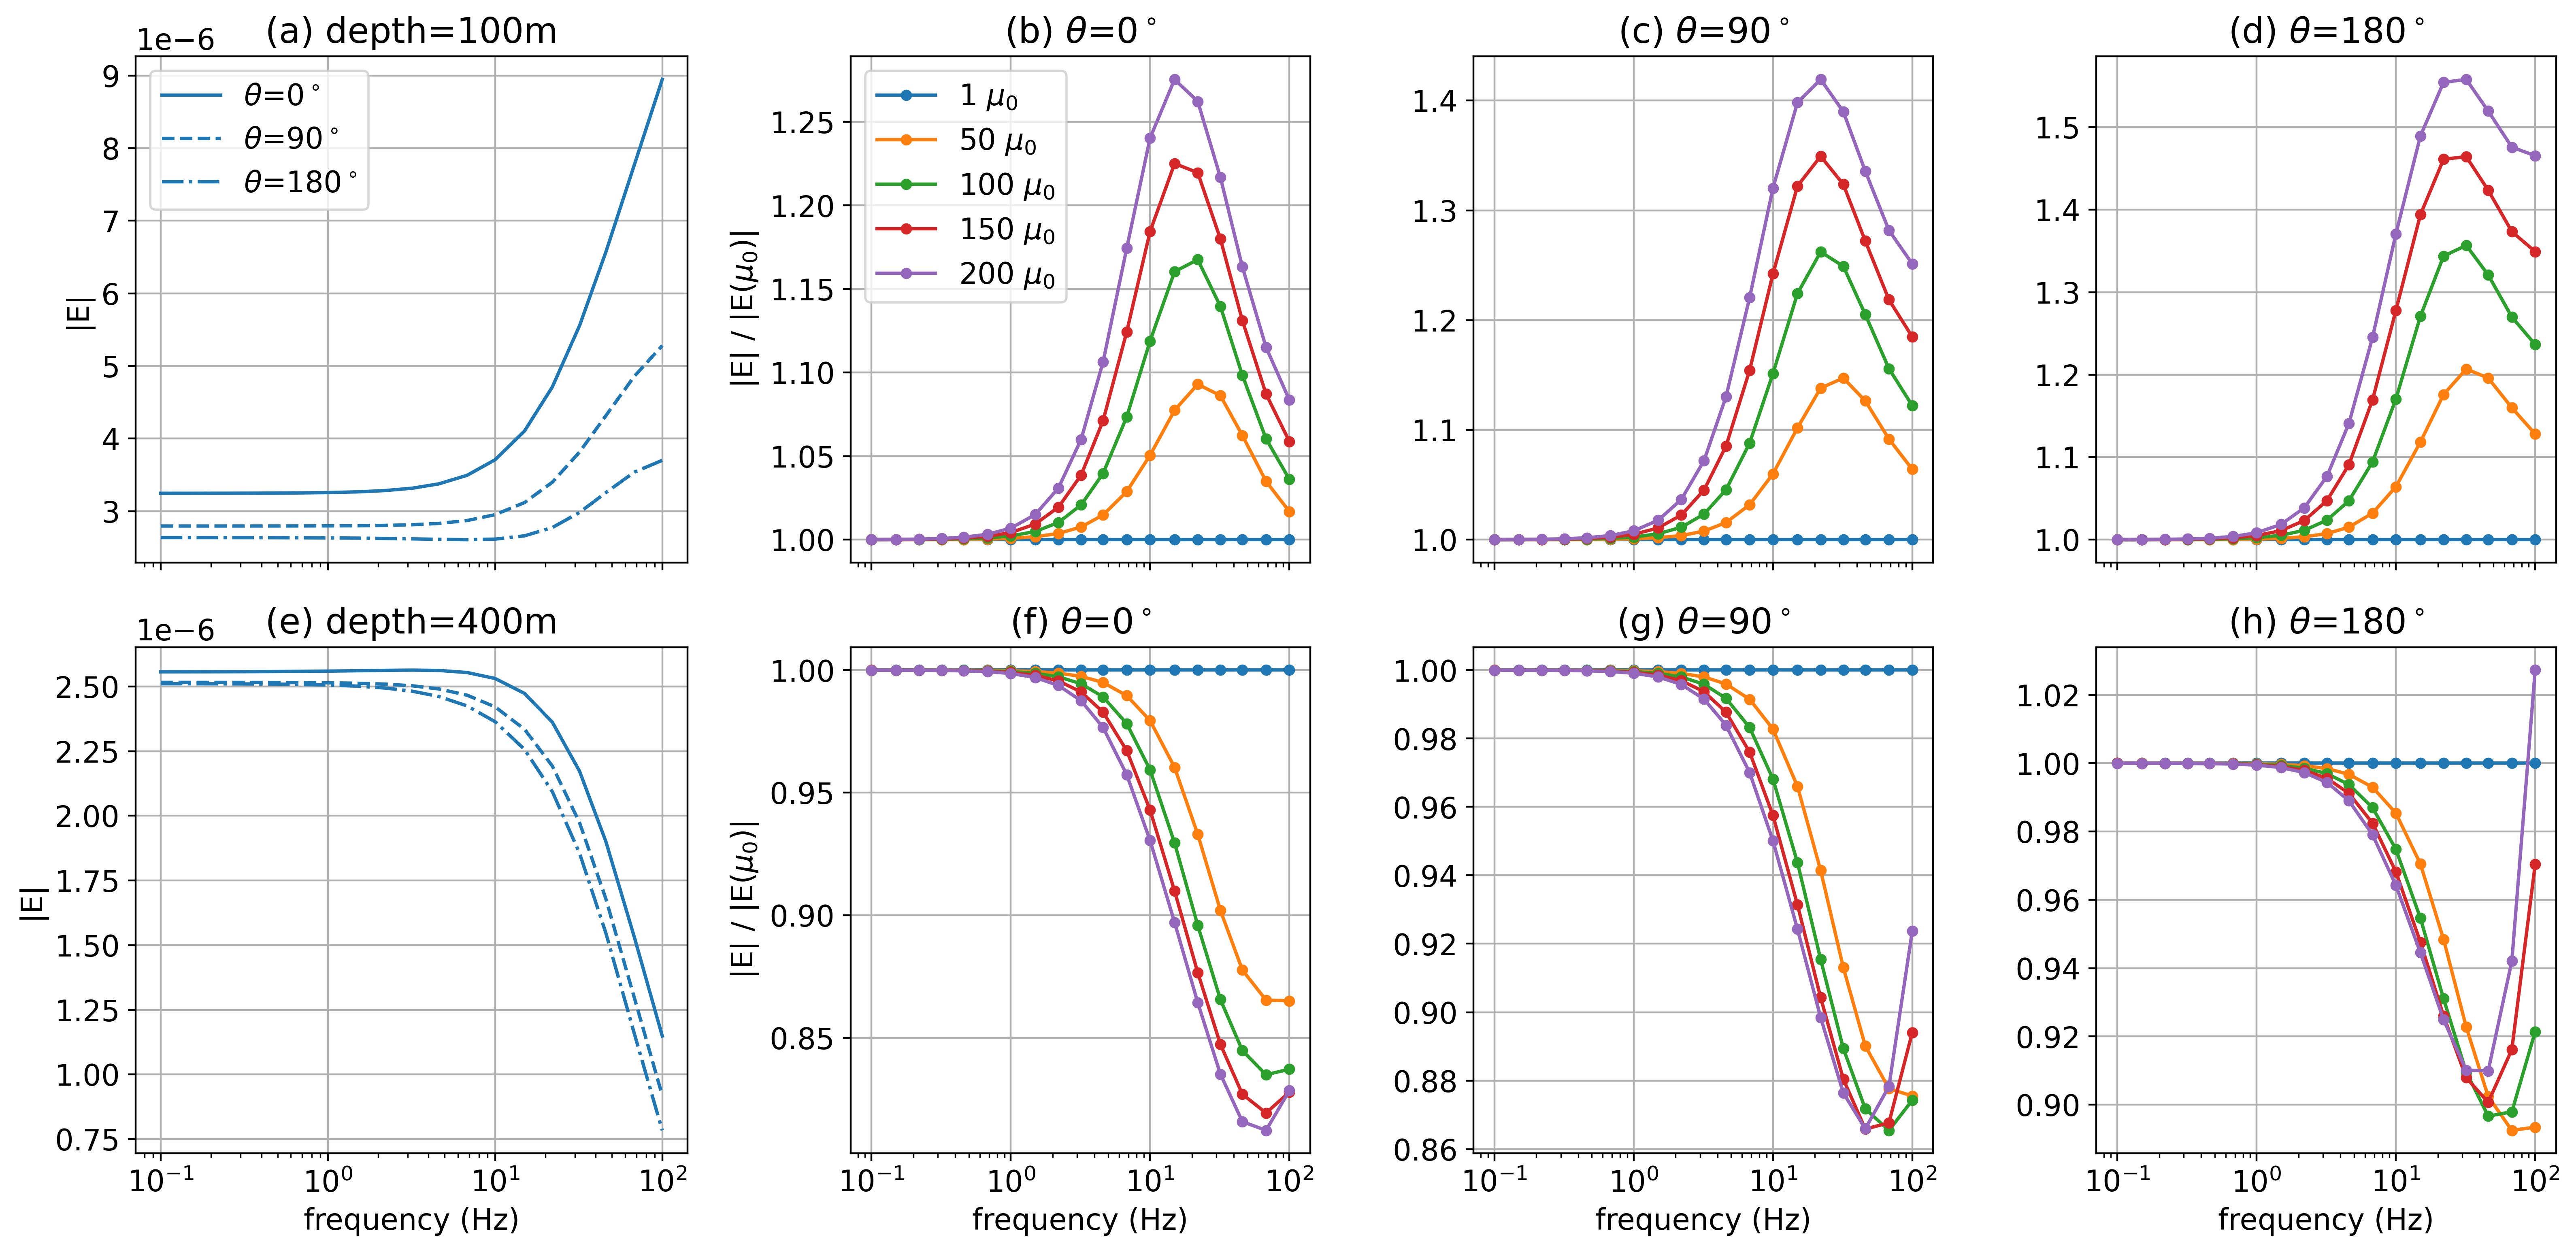
\includegraphics[width=\textwidth]{figures/excitation-freq.png}
    \end{center}
\caption{
    Amplitude of the average electric field over a test volume that is the same as was used in Figure \ref{fig:excitation-time-integrated}. The different line-styles in (a) and (e) indicate different azimuths for the non-permeable well ($\mu_0$). Panels (b), (c), and (d) show the ratio of the amplitude of the electric field with respect to the non-permeable well ($\mu=\mu_0$) for the test volume centered at a depth of 100m. Panels (f), (g) and (h) show the ratios of the electric field amplitude for the test volume centered at 400m depth.
}
\label{fig:excitation-freq}
\end{figure}





Interestingly, for a deeper test volume, permeability has the opposite effect and reduces the average electric field. This is consistent with the currents shown in Figure \ref{fig:fdem-cross-section-currents-real} where we see the total currents point away from the well at depth, while the anomalous currents in \ref{fig:fdem-cross-section-currents-real}(d) point towards the well. At the highest frequencies, there are reversals of currents at depth that can be seen at 100 Hz in Figure \ref{fig:fdem-cross-section-currents-real}. When the direction of the total and anomalous currents are the same, the response can then be enhanced, as seen at 100Hz in Figure \ref{fig:excitation-freq}(h). A reduction in the amplitude of the electric field as the permeability of the well is increased was not observed in the time-domain (Figure \ref{fig:excitation-time-integrated}). If, however, we subtract the galvanic response from the frequency domain results and isolate the inductive response, we obtain the results in Figure \ref{fig:excitation-freq-subtract-dc}. At both depths, there is an enhancement of the average electric field for frequencies below 20 Hz. This is consistent with the currents and anomalous currents in Figures \ref{fig:fdem-cross-section-currents-subtract-dc} and \ref{fig:fdem-cross-section-currents-imag}. Permeability can enhance the inductive component of the EM response, but whether this translates to an overall increase or decrease in the amplitude fields depends upon both the galvanic and induced components.


\begin{figure}
    \begin{center}
    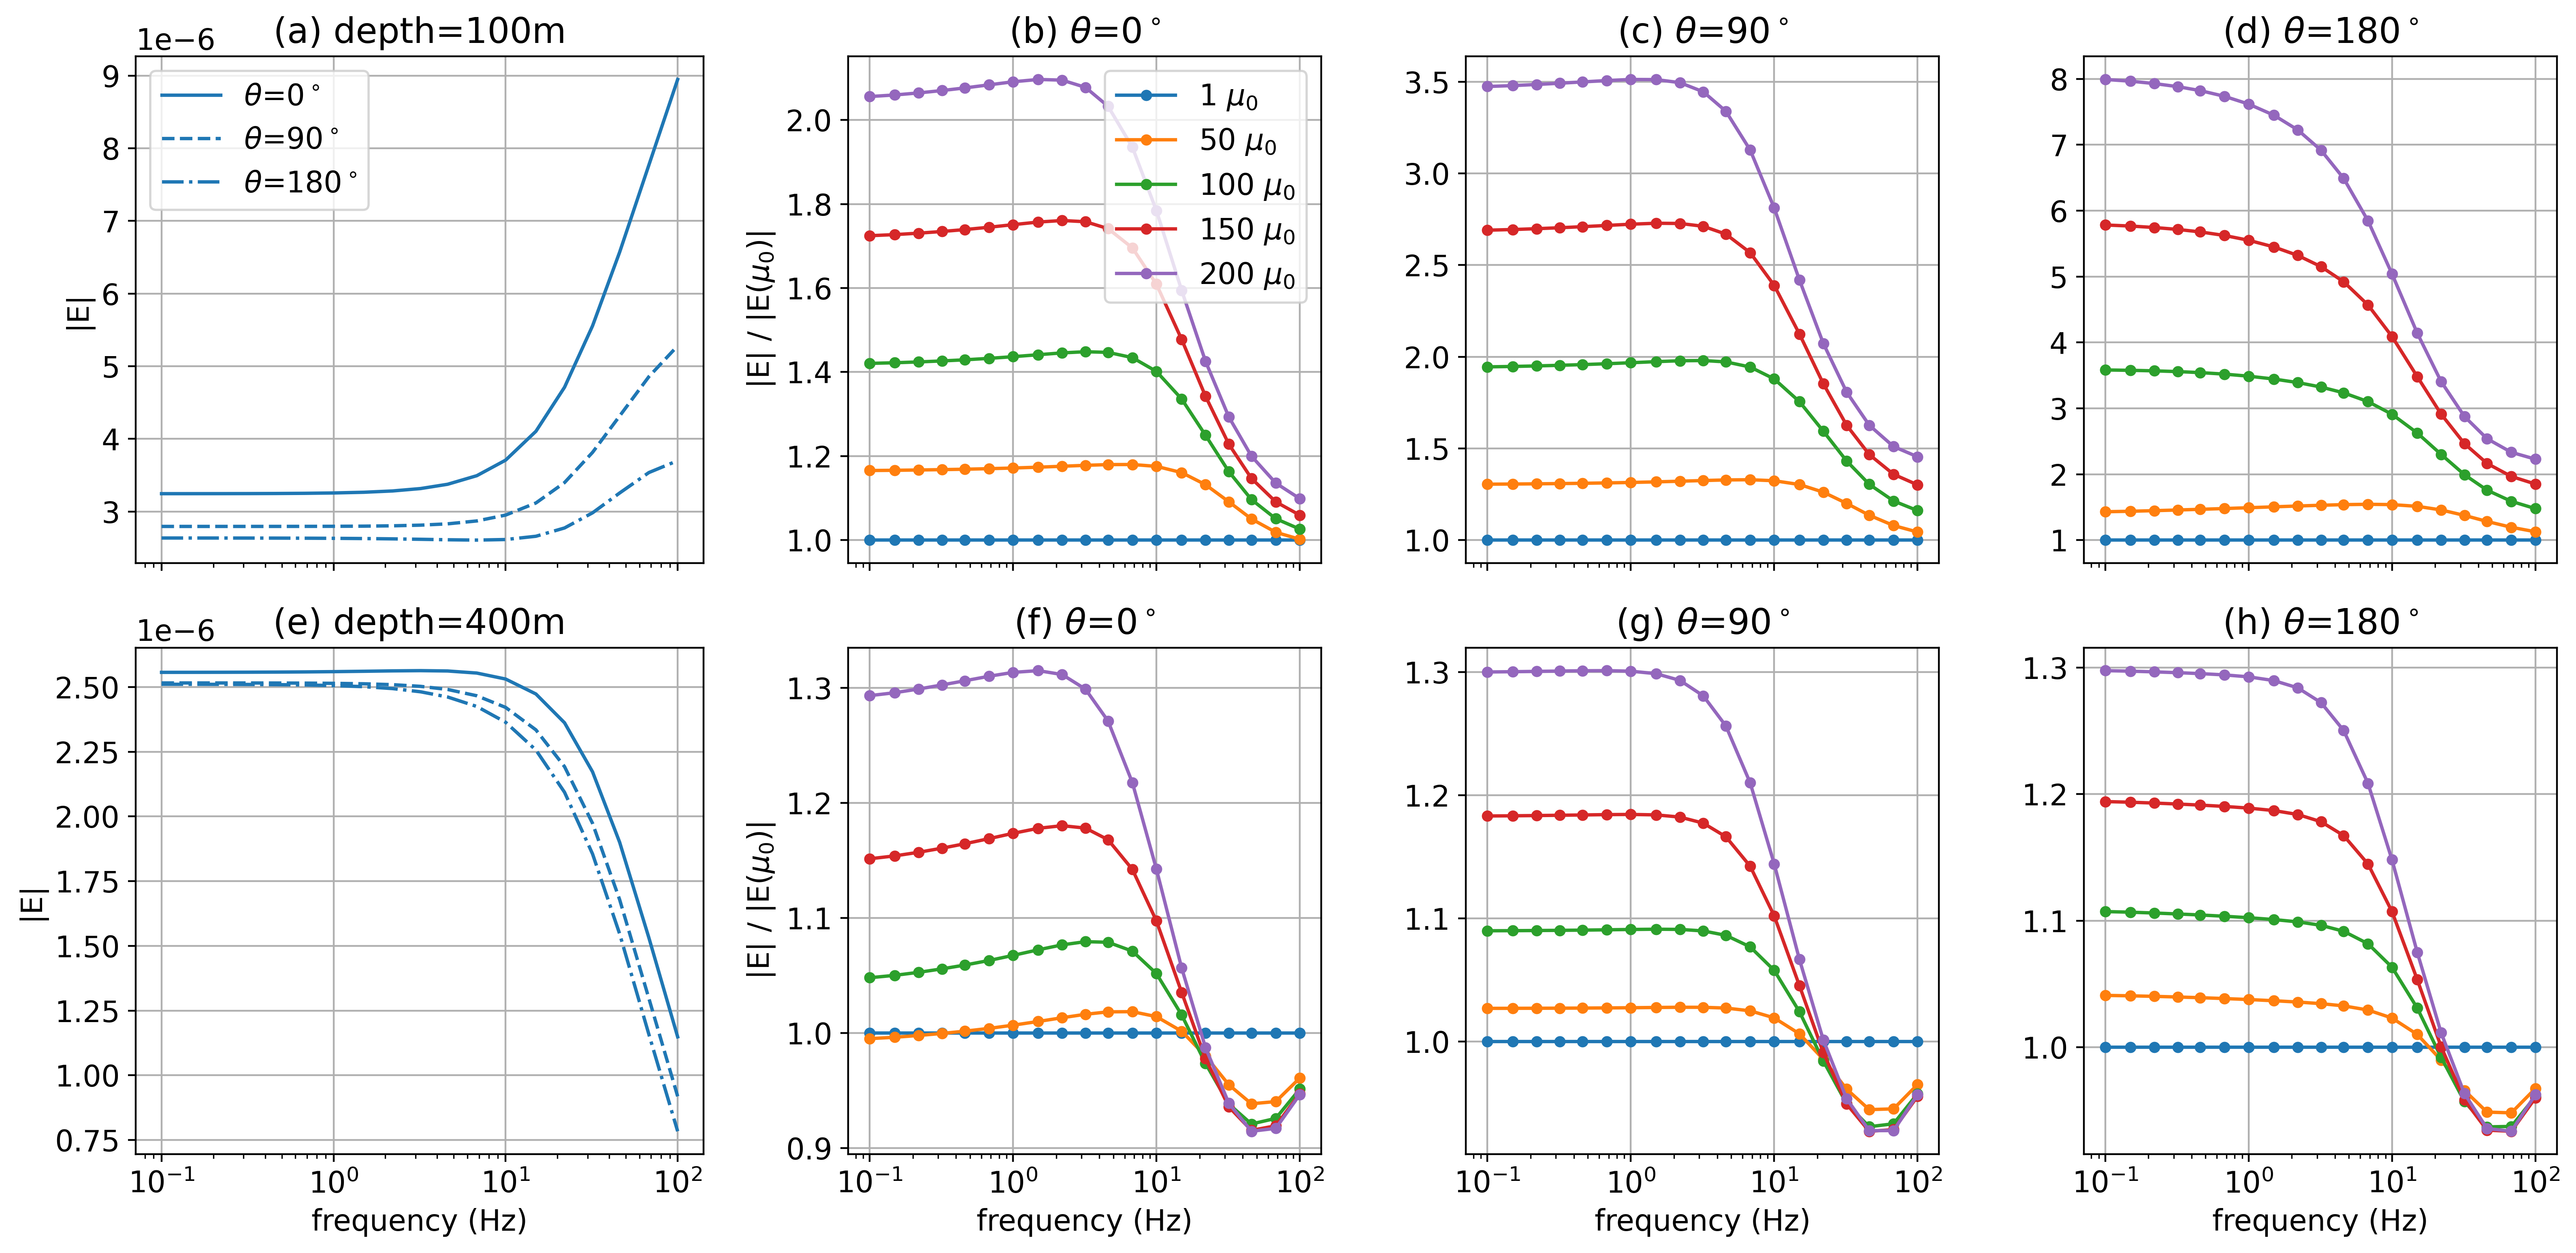
\includegraphics[width=\textwidth]{figures/excitation-freq-subtract-dc.png}
    \end{center}
\caption{
    Amplitude of only the inductive part of the electric field (total minus DC) over a test volume for the same experiment as shown in Figure \ref{fig:excitation-freq}.
}
\label{fig:excitation-freq-subtract-dc}
\end{figure}





\subsection{Currents within the casing}
To visualize the impacts of permeability on the currents in the casing, we zoom in to the casing wall and plot the currents at a range of frequencies. In Figure \ref{fig:fdem-casing-currents-real} we show (a) the DC response for a conductive casing, and (b) the inductive component of the real response, computed by subtracting the DC currents from the real component of the total currents at each frequency. The bottom row similarly shows the real component of the currents for a conductive, permeable casing ($\mu_r = 150$). Figure \ref{fig:fdem-casing-currents-imag} shows the imaginary component of the currents.

In comparing with the time-domain images in Figure \ref{fig:tdem-casing-currents}, we see that high-frequencies in the inductive part of the real component (Figure \ref{fig:fdem-casing-currents-real}) are similar in geometry and amplitude to the early times. The response at low frequencies is similarly analogous to later times, and we can again observe the poloidal current system in the permeable well. Again note that directions are opposite to the time domain because of the Fourier transform convention.


\begin{figure}
    \begin{center}
    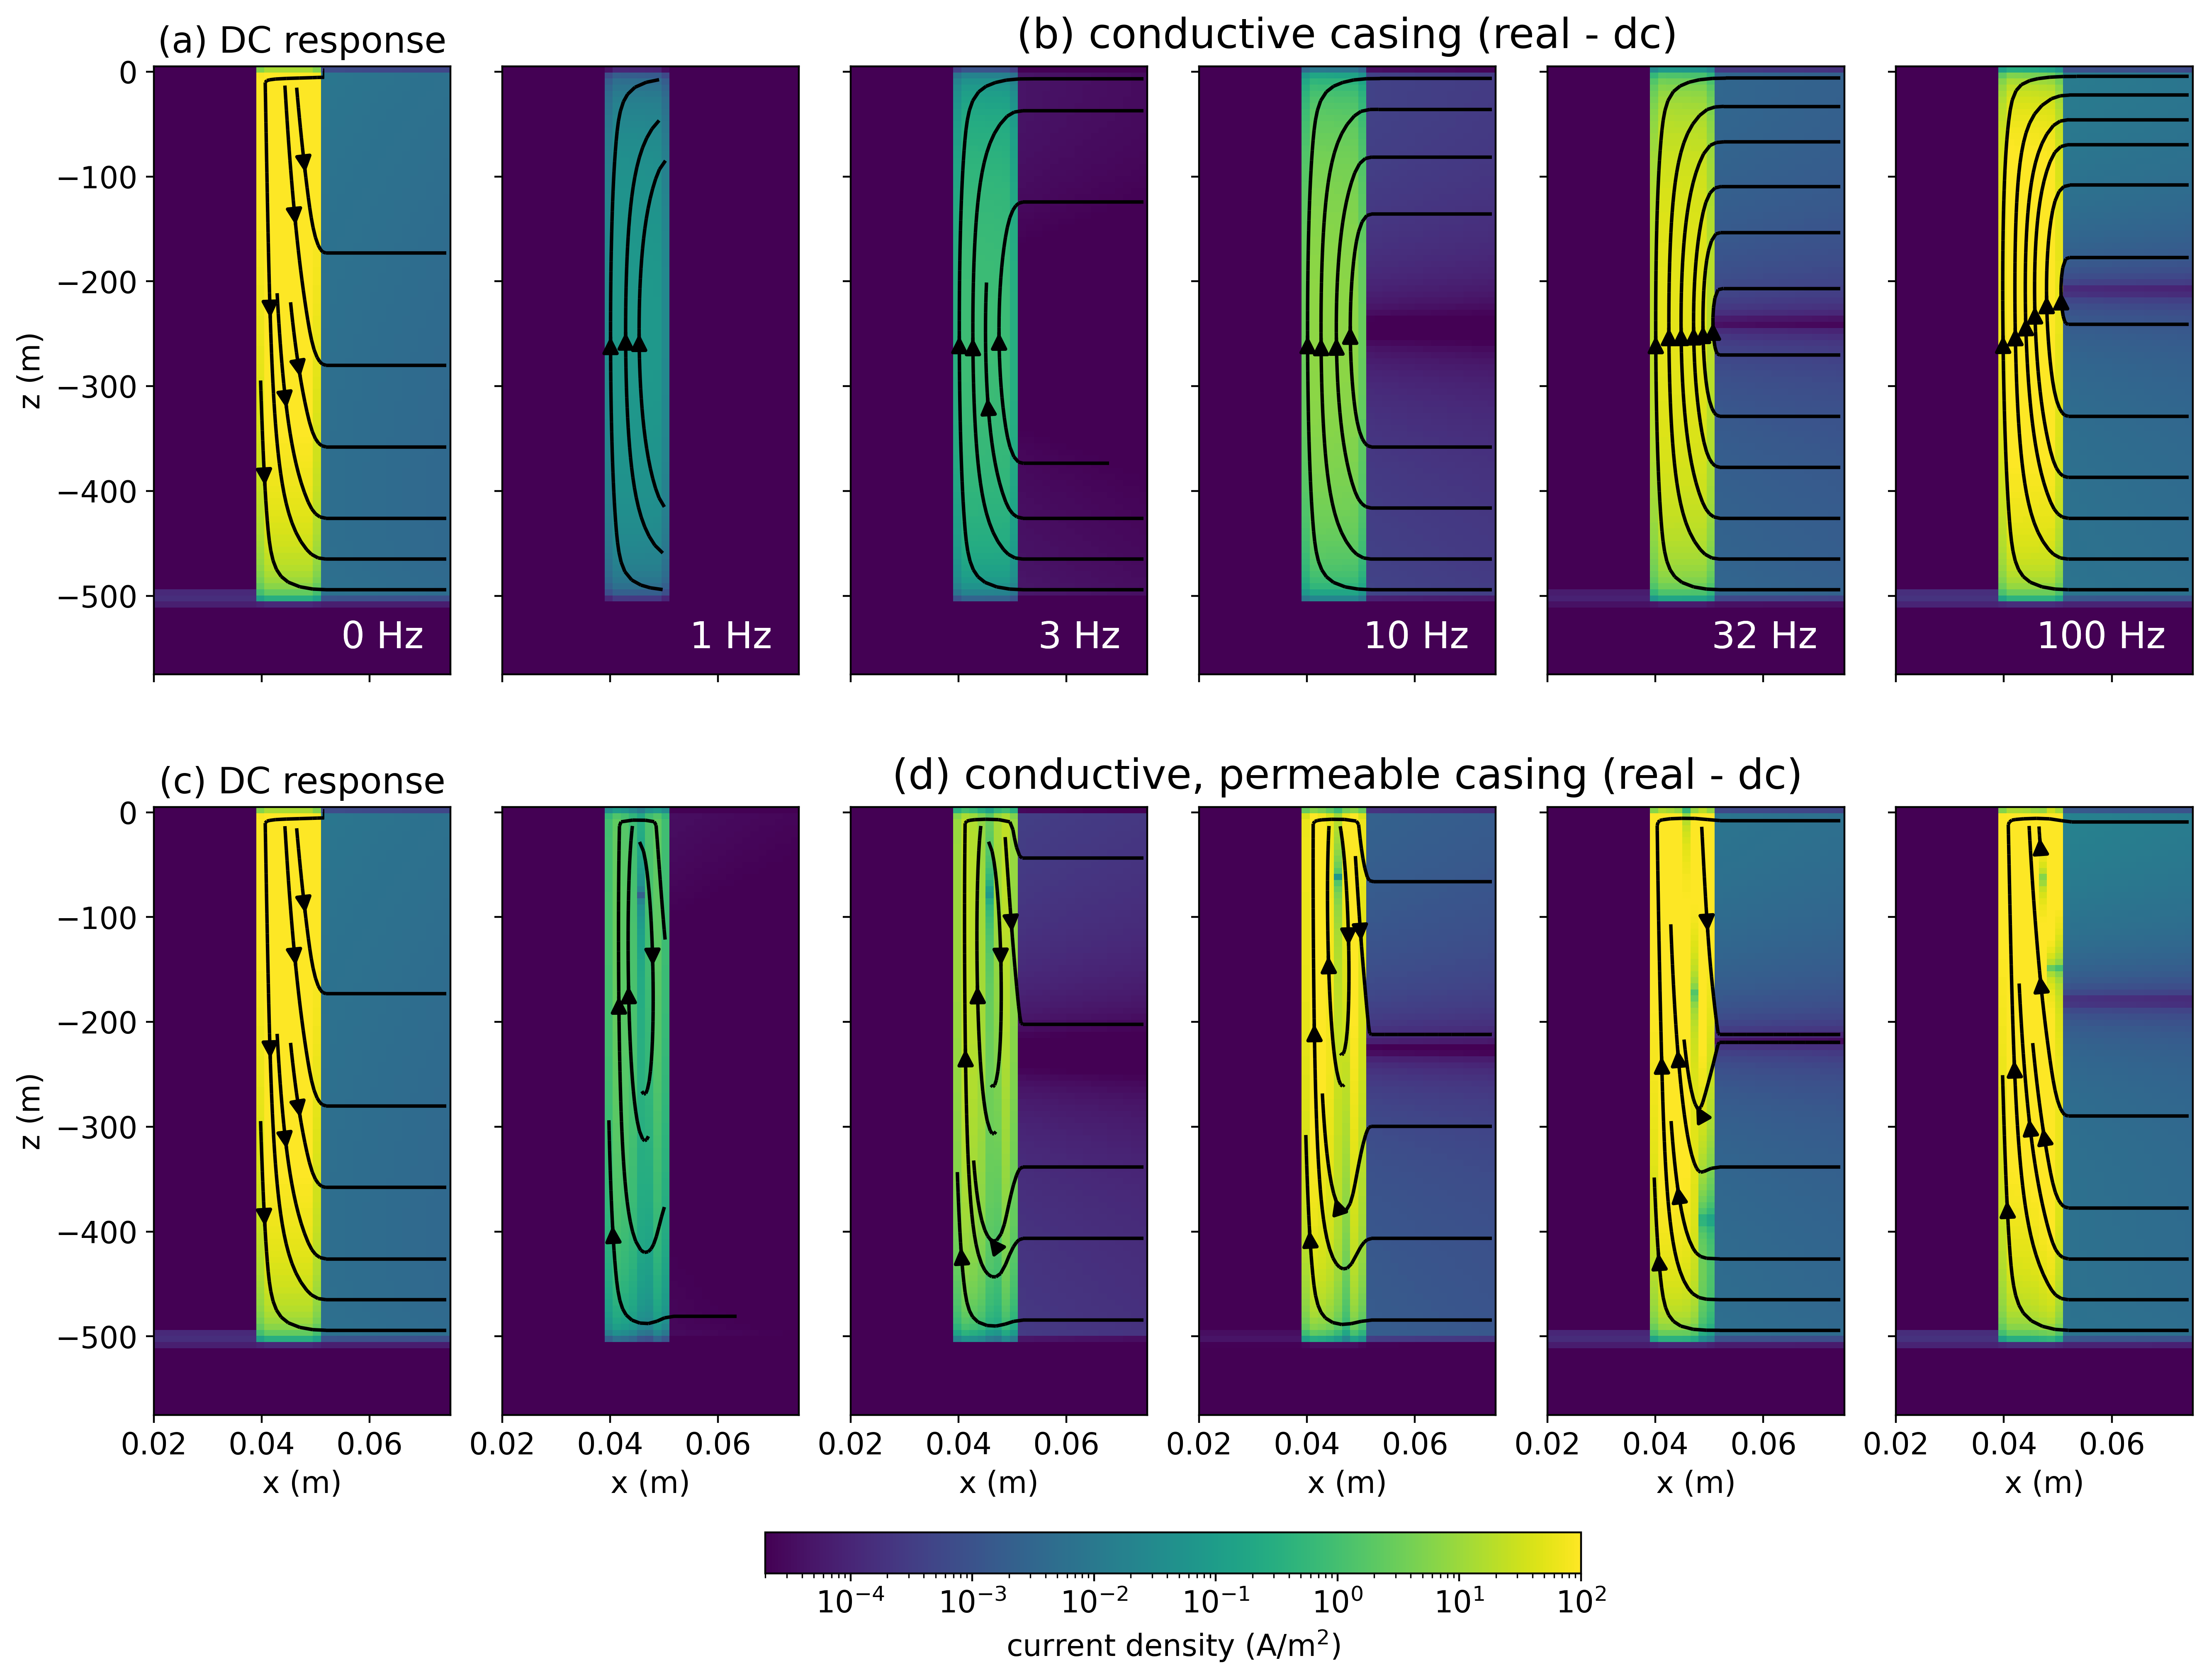
\includegraphics[width=1\textwidth]{figures/fdem-casing-currents-real.png}
    \end{center}
\caption{
    Cross sections of DC current density within (a) a conductive casing ($5\times10^6$ S/m, $\mu_0$) and (c) a conductive, permeable casing ($5\times10^6$ S/m, $150\mu_0$). The cross sections in (b) and (d) show the inductive part of the real current density (total - DC).
}
\label{fig:fdem-casing-currents-real}
\end{figure}






\begin{figure}
    \begin{center}
    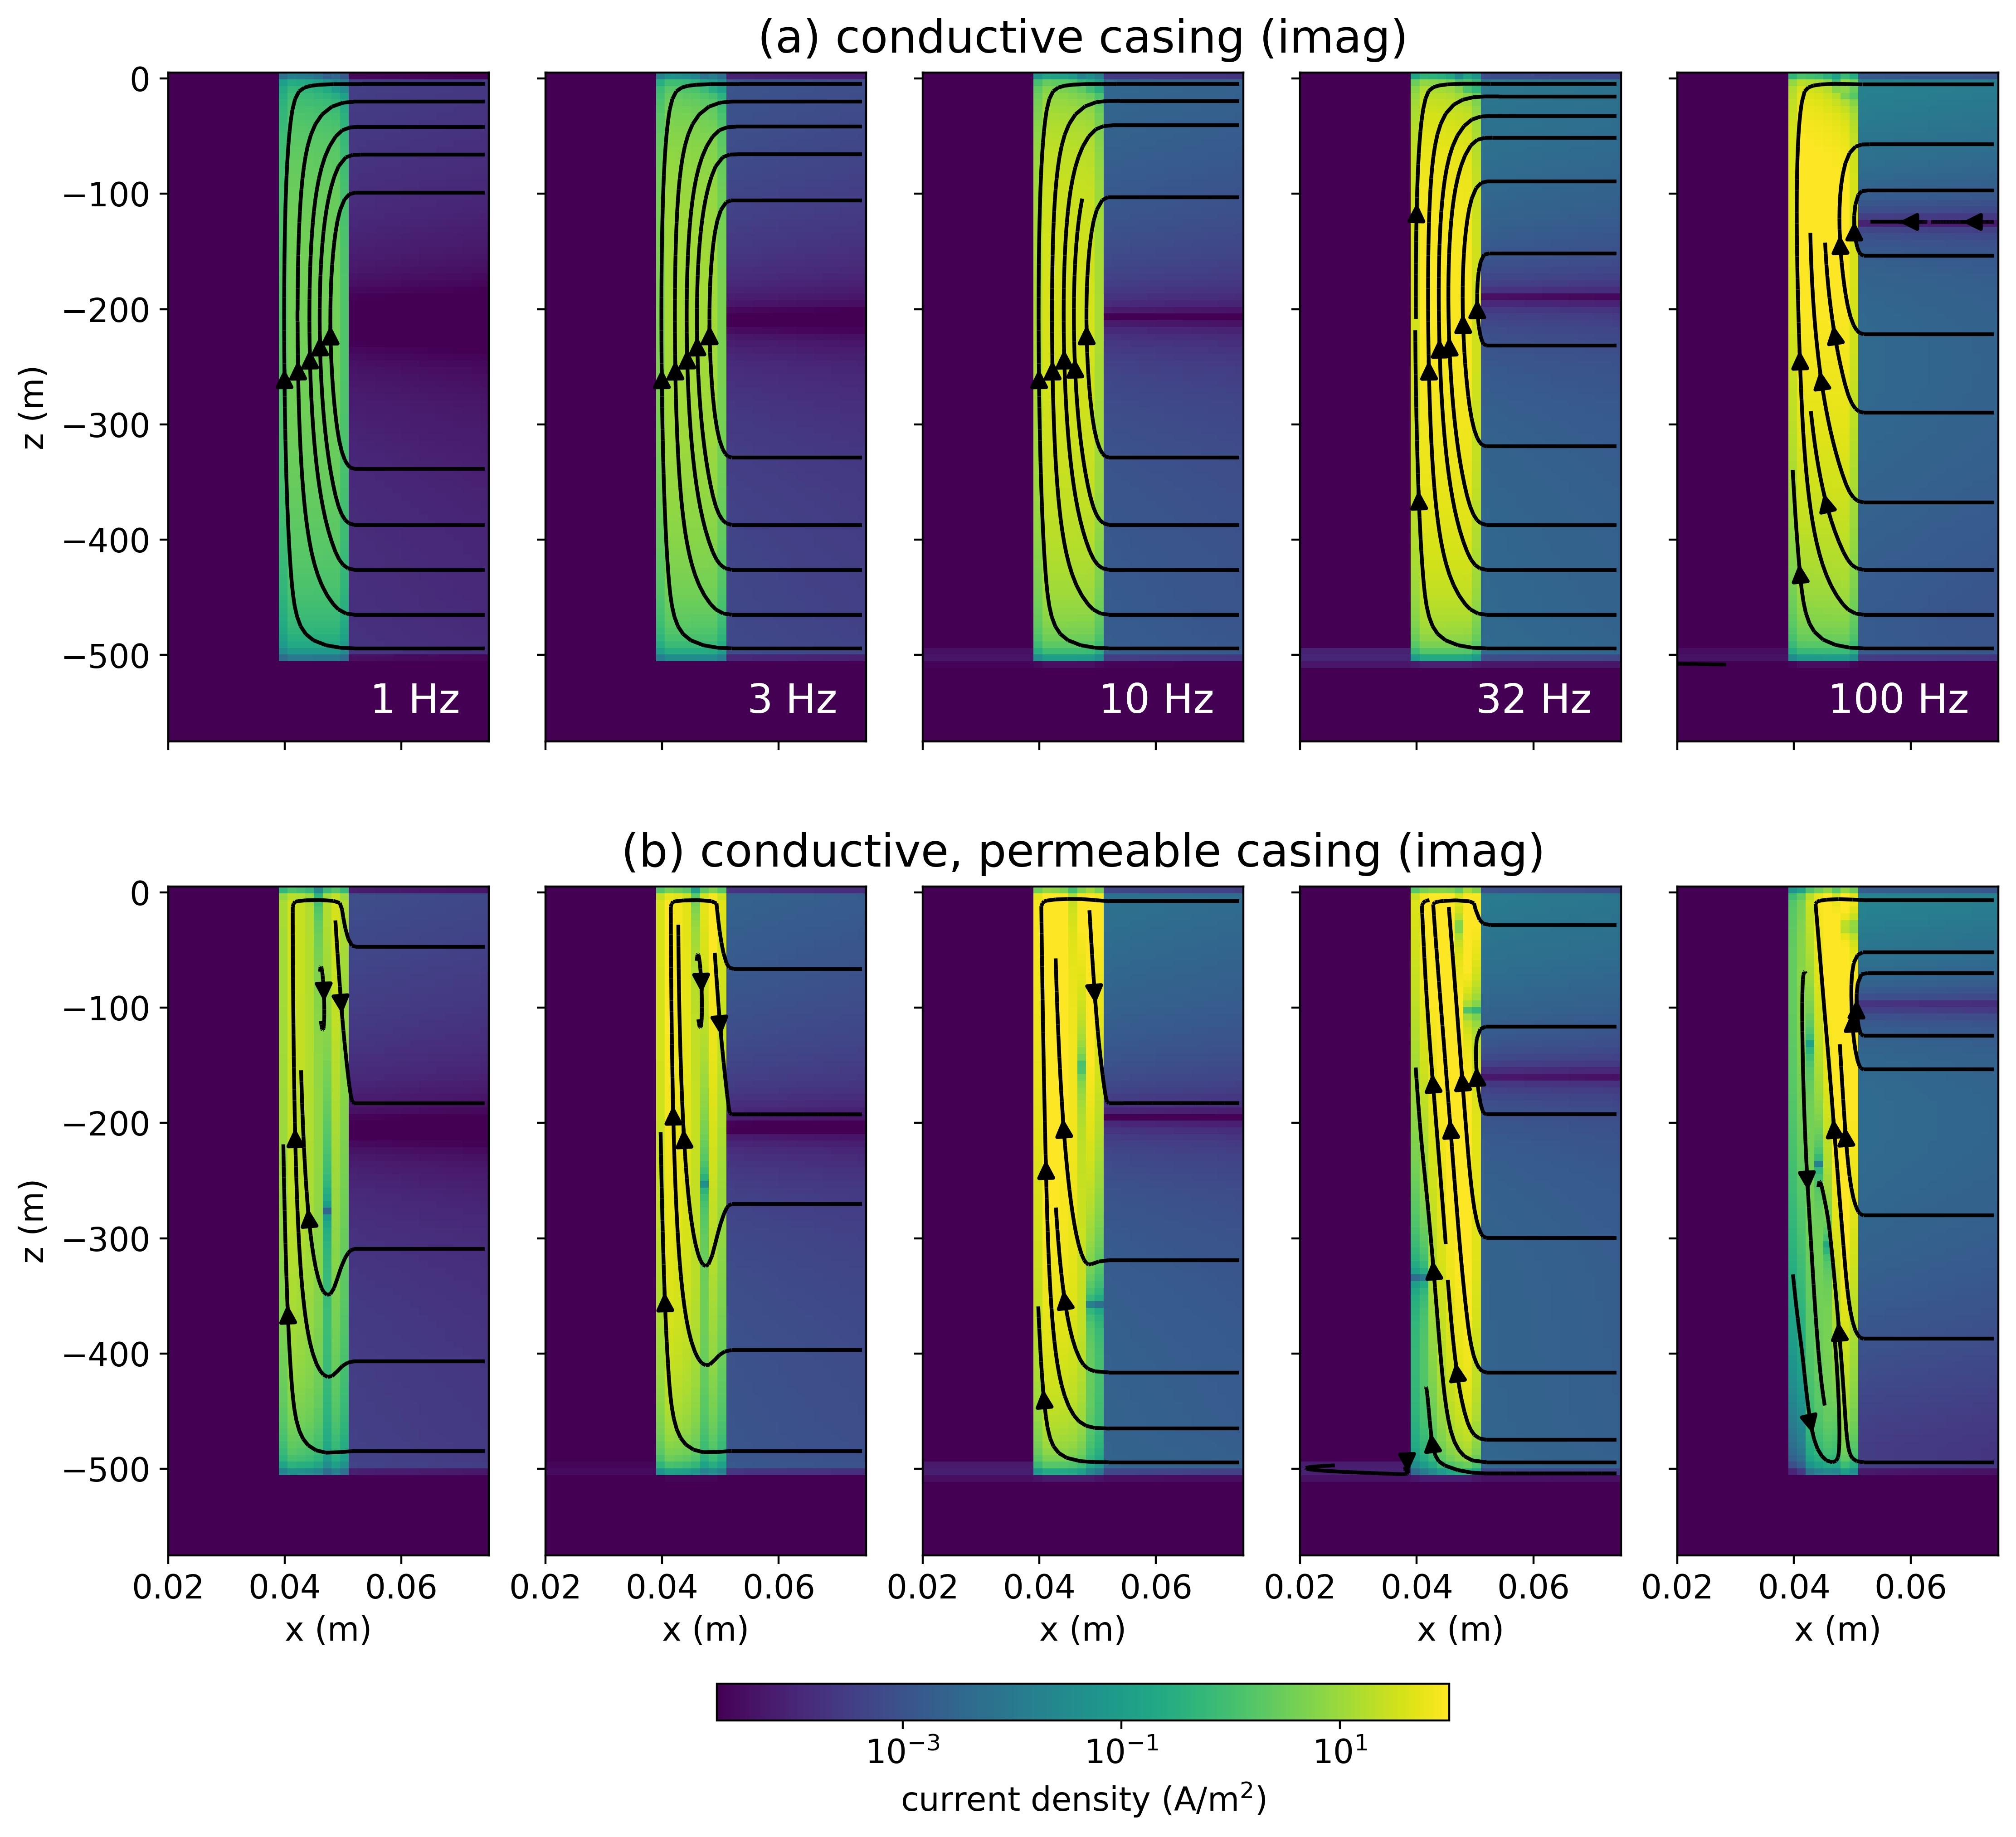
\includegraphics[width=0.8\textwidth]{figures/fdem-casing-currents-imag.png}
    \end{center}
\caption{
    Cross sections of the imaginary part of the current density within (a) a conductive casing ($5\times10^6$ S/m, $\mu_0$) and (b) a conductive, permeable casing ($5\times10^6$ S/m, $150\mu_0$).
}
\label{fig:fdem-casing-currents-imag}
\end{figure}





\subsection{Explaining the poloidal current system}
The same reasoning as we used to explain the poloidal current system in the time domain holds for the frequency domain. Replacing the time-domain fields and fluxes in equation \ref{eq:permeability-ampere-no-source} with frequency domain variables, we have
\begin{equation}
\nabla \times \vec{B} = \nabla \ln \mu_r \times \vec{B} + \mu\sigma\vec{E}
\label{eq:permeability-ampere-no-source-freq}
\end{equation}


In Figure \ref{fig:magnetization-term-freq}, we plot the real and imaginary component of the magnetic flux density in the vicinity of the casing at two different frequencies 1 Hz and 10 Hz. Examining equation \ref{eq:permeability-ampere-no-source-freq}, we know that at DC (0 Hz), there is no influence of $\vec{B}$ on $\vec{E}$. So although the magnetization term in equation \ref{eq:permeability-ampere-no-source-freq} is non-zero when the casing is permeable, this portion of the response has no influence on the currents or electric fields (by Faraday's law). So we subtract off the DC response and focus our attention on the inductive parts of $\vec{B}_\theta$ in Figure \ref{fig:magnetization-term-freq} (c-f) to understand how the permeability of the casing impacts the EM response. The real, inductive part of the magnetic flux density (c-d) is positive along the outer edge of the casing and therefore contributes to a downward-going magnetization current. This is similarly true for the imaginary component.


\begin{figure}
    \begin{center}
    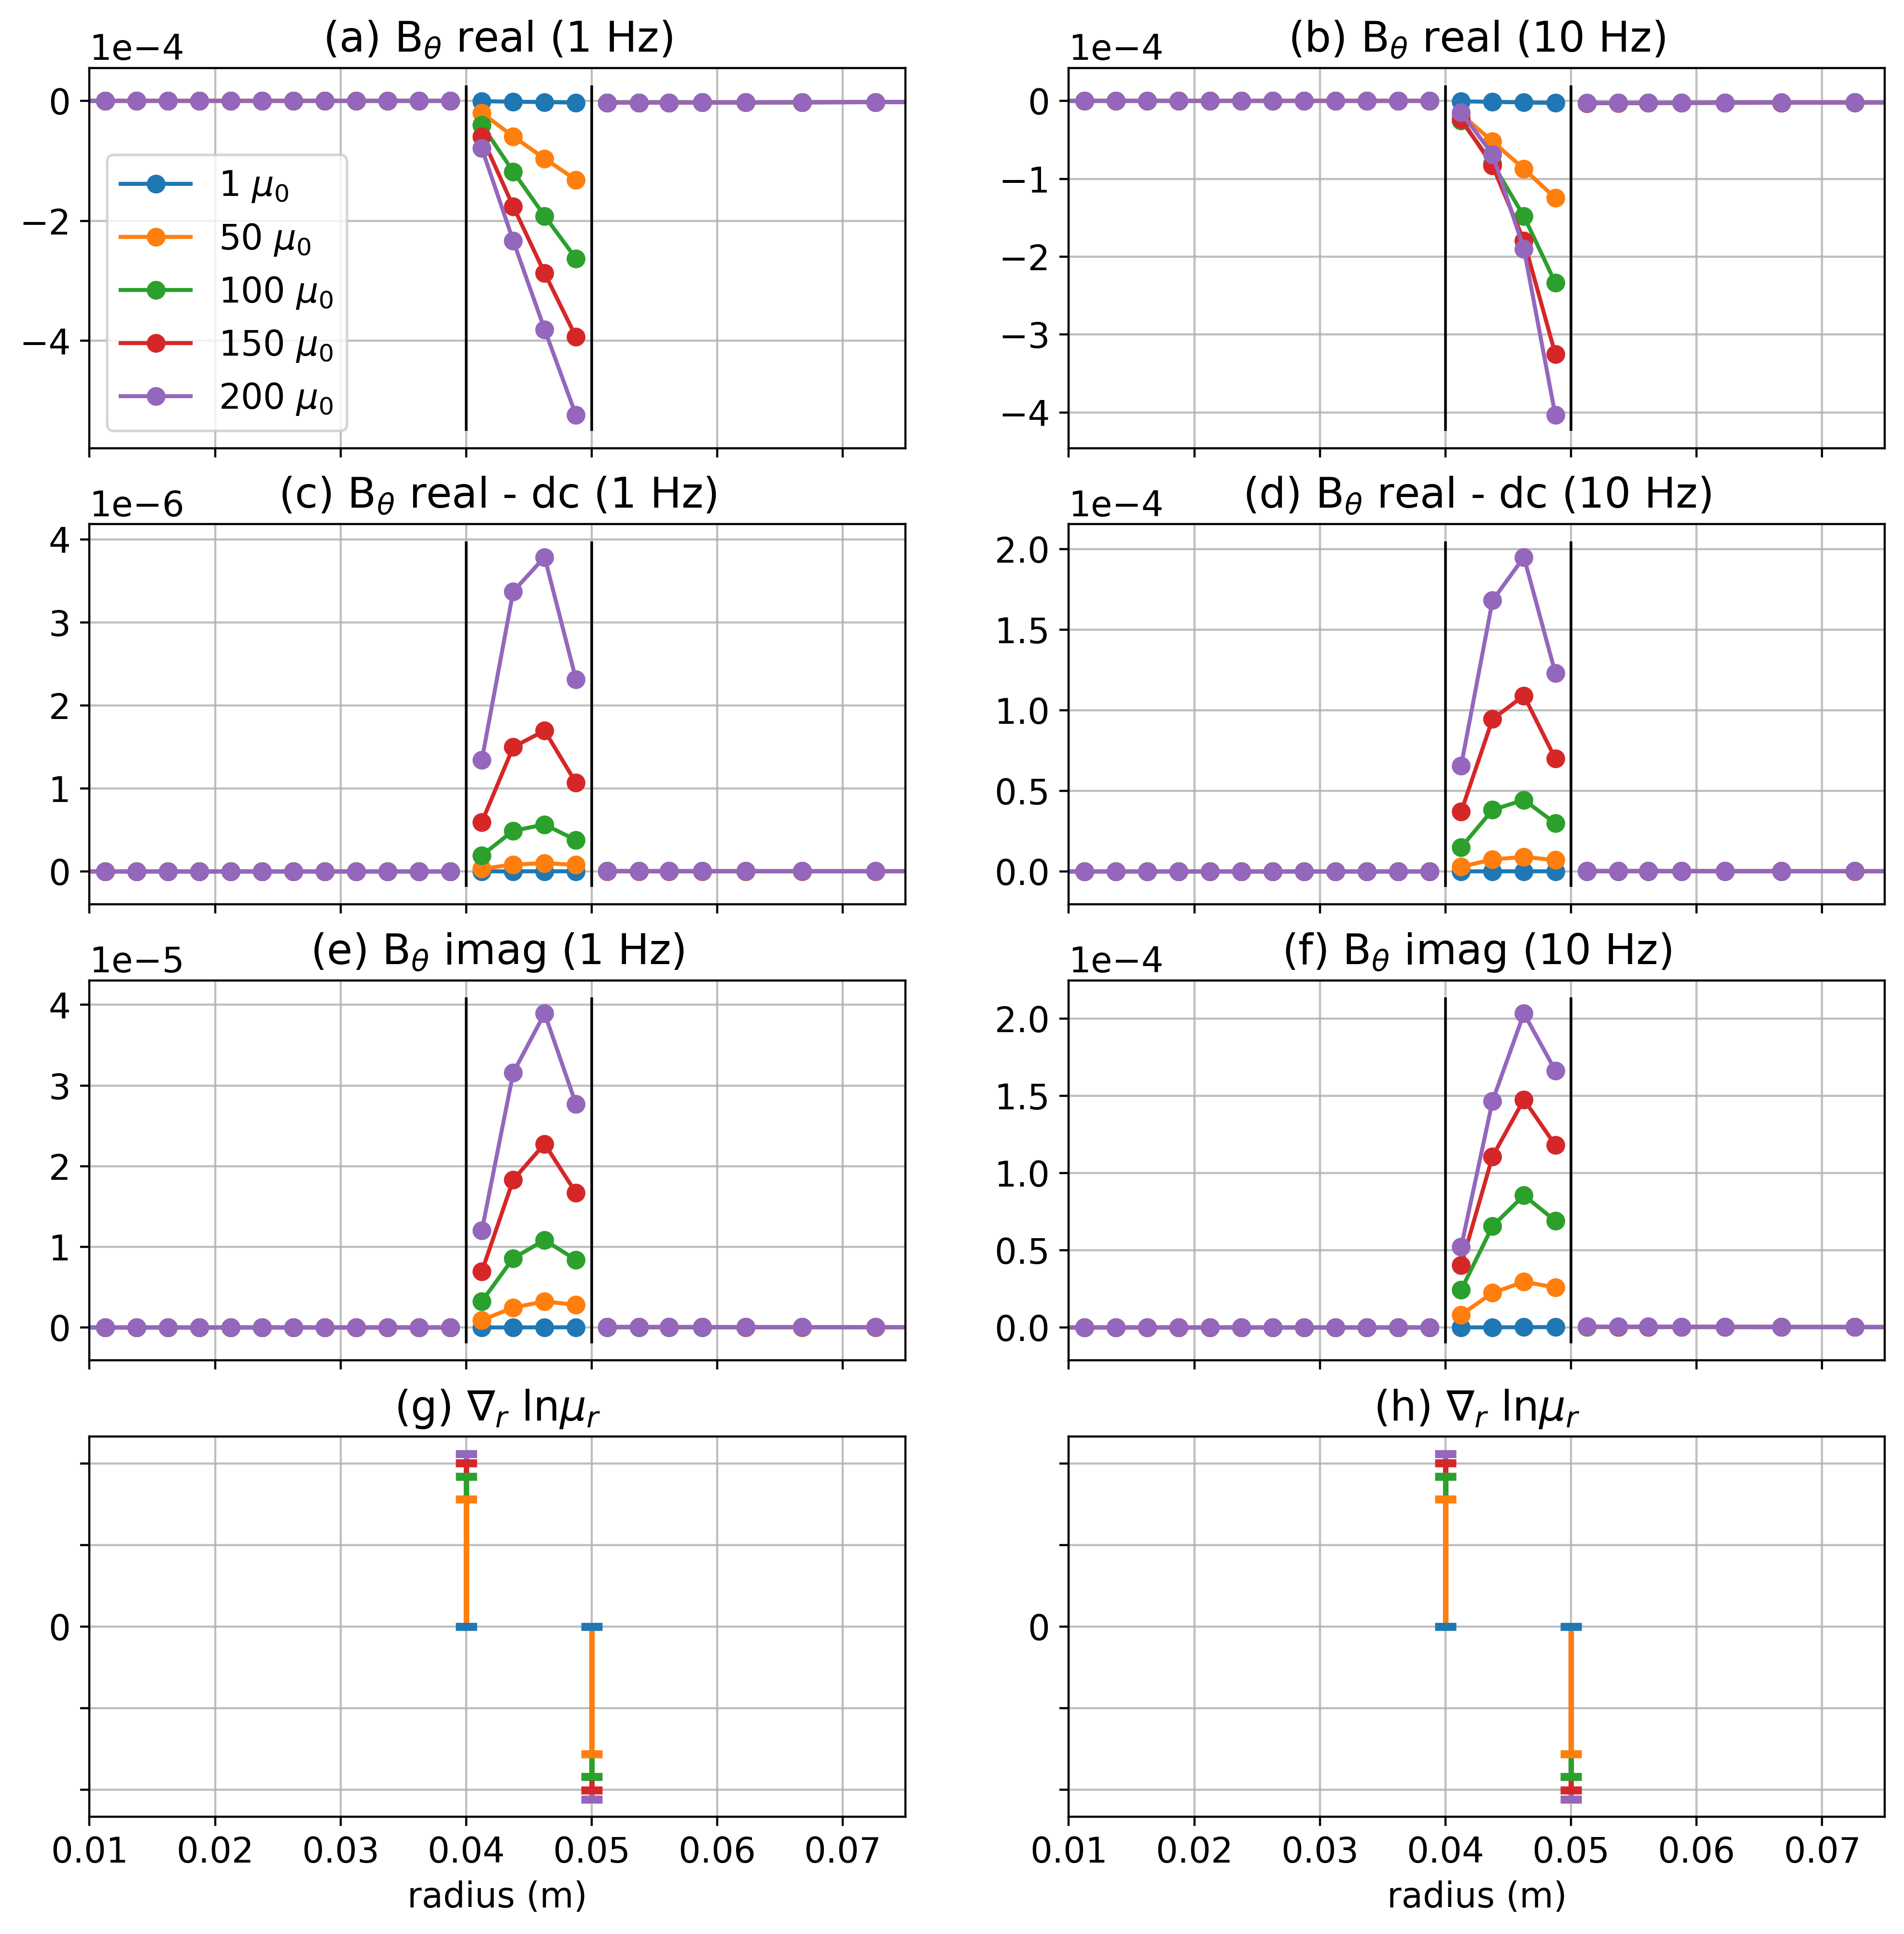
\includegraphics[width=\textwidth]{figures/magnetization-term-freq.png}
    \end{center}
\caption{
    (a-b) Real part of the azimuthal component of the magnetic flux at 1 Hz and 10 Hz, respectively.
    (c-d) Inductive part of the real component of the magnetic flux (real - dc).
    (e-f) Imaginary component of the magnetic flux.
    (g-h) Radial component of $\nabla \ln \mu_r$.
}
\label{fig:magnetization-term-freq}
\end{figure}





